% ===========================================================================
%  ESField v7.1 — Publication-ready manuscript
%  "Topology-Aware Inference Guidance Enables Hydration-Site-Occupying
%   Molecular Generation, But Rigid Anchor Fixation Compromises Binding Affinity"
%
%  Compile with: pdflatex ×2
% ===========================================================================

\documentclass[11pt,letterpaper]{article}

% ── Packages ──────────────────────────────────────────────────────────────
\usepackage[utf8]{inputenc}
\usepackage[T1]{fontenc}
\usepackage{amsmath,amssymb}
\usepackage{booktabs}
\usepackage{graphicx}
\usepackage[colorlinks=true,linkcolor=blue,citecolor=blue,urlcolor=blue]{hyperref}
\usepackage{natbib}
\usepackage{caption,subcaption}
\usepackage{multirow}
\usepackage{geometry}
\geometry{margin=1in}
\usepackage{float}
\usepackage{xcolor}
\usepackage{siunitx}
\usepackage{enumitem}

% bioRxiv-style title block
\makeatletter
\renewcommand{\@maketitle}{%
  \begin{center}%
    {\LARGE\bfseries\@title\par}%
    \vskip 1.5em%
    {\large\@author\par}%
    \vskip 1em%
    {\normalsize\@date\par}%
  \end{center}%
  \vskip 1em%
}
\makeatother

\begin{document}

\title{Topology-Aware Inference Guidance Enables Hydration-Site-Occupying\\
       Molecular Generation, But Rigid Anchor Fixation Compromises\\
       Binding Affinity}

\author{Author Name(s)\\[3pt]
        \small\textit{Institution(s)}\\[3pt]
        \small\textit{Correspondence: corresponding.author@institution.edu}}

\date{}

\maketitle

% ===========================================================================
%  ABSTRACT
% ===========================================================================
\begin{abstract}
Structure-based molecular generation models have demonstrated promising
capabilities in designing ligands conditioned on protein binding sites, yet
existing approaches systematically ignore crystallographic water
molecules---particularly high-energy waters (HEWs) whose displacement can
contribute 0.5--2.0~kcal/mol to binding free energy.  We previously showed
that coordinate-only latent guidance (ESField v6-D.2) cannot induce HEW site
occupancy, with 0/180 generated molecules achieving direct water displacement
across three diverse PDBbind pockets.  Here, we introduce ESField v7.1, a
two-stage topology-aware generation framework that decomposes the problem into
(i) Phase~1 fragment growth at HEW sites under strong site-compatibility energy
guidance ($\lambda=5.0$) with Kinetic Trajectory Shaping (early boost, late
damping), and (ii) Phase~2 hard-fixation of anchor atoms followed by full
molecule completion under weak guidance.  Across 10 PDBbind pockets with diverse
HEW environments, v7.1 achieves DirectOcc $> 0\%$ in 7/10 pockets (versus 0\%
baseline), representing the first demonstration of inference-time HEW site
control in a flow-matching generator.  Molecular diversity improves by
27--45\% (Vendi score).  Ablation experiments confirm $\lambda=5.0$ as the
optimal Phase~1 guidance strength and show that hard anchor fixation produces
occupancy rates comparable to soft harmonic restraint (15.1\% vs.\ 14.2\%).
Critically, however, HEW-occupying molecules do \emph{not} achieve superior
Vina docking scores compared to non-occupying molecules; in the 3mfw pocket,
the occupied group trends toward \emph{worse} scores ($p=0.067$, Cliff's
$\delta=+0.47$).  These results demonstrate that topology-level control can
successfully enforce water-site utilization, but that rigid anchor fixation may
compromise overall binding optimization---a previously unrecognized
``occupancy--affinity paradox'' that motivates flexible anchor annealing
strategies for reconciling site-level control with global conformational
quality.

\medskip
\noindent\textbf{Keywords:} structure-based drug design, 3D molecular
generation, hydration sites, high-energy water, flow matching, inference-time
guidance, kinetic trajectory shaping, water displacement
\end{abstract}

% ===========================================================================
%  INTRODUCTION
% ===========================================================================
\section{Introduction}

\subsection{Hydration Sites as Design Opportunities in Drug Discovery}

Water molecules at protein--ligand interfaces play a critical, dual role in
molecular recognition~\cite{ladbury1996,spyrakis2017}.  While many interfacial
waters are structurally conserved and contribute to binding affinity through
hydrogen-bond networks, a subset---termed high-energy waters (HEWs) or
``unhappy'' waters---reside in energetically unfavorable local
environments~\cite{young2007,abel2008}.  Displacing these HEWs with compatible
ligand functional groups can yield substantial gains in binding free energy,
with estimates ranging from 0.5 to 2.0~kcal/mol per displaced
water~\cite{michel2009,wang2015}.  Computational methods for predicting
hydration sites and their thermodynamic signatures are now well-established,
including WaterMap~\cite{abel2008}, Grand Canonical Monte Carlo
(GCMC)~\cite{ross2012}, Grid Inhomogeneous Solvation Theory
(GIST)~\cite{nguyen2012}, and 3D-RISM~\cite{luchko2010}.  However, incorporating
this information as explicit \emph{design constraints} during \emph{de novo}
molecular generation remains an open challenge~\cite{spyrakis2017}.

\subsection{The Water-Blindness of 3D Generative Models}

Recent advances in 3D-aware molecular generation---including
TargetDiff~\cite{guan2023}, DiffSBDD~\cite{schneuing2024}, DecompDiff~\cite{guan2023decomp},
DrugFlow~\cite{drugflow2024}, and FLAG~\cite{zhang2024flag}---have enabled the
generation of drug-like molecules directly conditioned on protein pocket
geometry.  These models learn to sample atom types and coordinates from a
distribution over protein--ligand complexes, achieving impressive validity rates
and binding pose accuracy.

A key limitation, however, is that these models are trained on crystallographic
structures from the Protein Data Bank~\cite{berman2000} that rarely retain
explicit water molecules at the binding interface.  Consequently, the learned
distribution encodes no information about which pocket regions should be
occupied by ligand atoms versus water molecules.  The model has no incentive to
displace a HEW---it may equally well place a methyl group \emph{next to} the
water site, leaving the energetically unfavorable water in place and forfeiting
a significant binding affinity opportunity.  We term this deficiency
\textbf{water-blindness}: the inability of current generators to distinguish
between water-occupied and water-displaceable regions of a binding pocket.

\subsection{Inference-Time Guidance: Promise and Limitations}

Inference-time guidance methods have emerged as a flexible paradigm for imposing
design objectives on pre-trained generators without
retraining~\cite{dhariwal2021,ho2022cfg,bansal2023}.  In the molecular domain,
this approach has been adopted in several forms.  Lai et al.~\cite{lai2025force}
demonstrated that incorporating MMFF94 force-field gradients during flow
matching sampling substantially improves binding affinity predictions and
reduces ligand strain energy by up to 75\%.  Lam et al.~\cite{lam2026metadiffusion}
introduced Metadiffusion, which applies Stein Variational Gradient Descent
(SVGD) repulsion as a meta-energy biasing layer on the Boltz-2 biomolecular
diffusion model, enabling controlled exploration of collective variables and
experimental data integration without retraining.  Li et al.~\cite{li2026kpe}
formalized Kinetic Path Energy (KPE) as a per-sample diagnostic of transport
cost in flow matching, and proposed Kinetic Trajectory Shaping (KTS)---a
phase-specific velocity modulation strategy that boosts early motion and damps
late-stage velocity to prevent memorization.  Griesbacher et
al.~\cite{griesbacher2026ebmol} introduced EBMol, an energy-based model that
learns an atom-additive scalar potential, demonstrating that fixing atomic
coordinates can steer conditional generation.  Additional guidance strategies
include pharmacophore-constrained generation~\cite{kpe2024} and
collective-variable-based enhanced sampling for molecular diffusion~\cite{nam2025cv}.

Critically, however, all of these methods operate on \emph{global} properties of
the generated structure (binding energy, RMSD, collective variables)---none
provides \textbf{site-type-level} control that distinguishes between chemically
distinct microenvironments (e.g., hydrophobic vs.\ polar-unsatisfied vs.\ mixed
hydration sites) within a single binding pocket.  This distinction is essential
for water-aware molecular design, where different hydration sites demand
different chemical responses from the ligand.

\subsection{The Topological Nature of Water Displacement}

Our earlier ESField v6-D.2 implementation~\cite{esfield2026} applied analytic
field-based coordinate guidance to nudge atoms toward HEW sites during
DrugFlow's ODE integration.  However, this ``coordinate-only'' approach failed
completely: across 180 molecules generated on three pockets, \emph{zero}
achieved direct HEW site occupancy.  The diagnosis was clear: coordinate nudging
alone cannot change atom types, add atoms, or reorganize local bonding
topology---it can only shift existing atoms by small amounts.  Water
displacement is fundamentally a \textbf{topological} problem, not a geometric
one: it requires placing chemically compatible atoms at specific locations where
they did not previously exist, which demands control over the generative process
during the early, topology-determining phase of denoising.

\subsection{This Work}

We introduce ESField v7.1, a \textbf{two-stage topology-aware inference guidance
framework} that addresses the fundamental limitation of coordinate-only
guidance.  Guided by the KPE insight that early denoising steps govern
topological decisions~\cite{li2026kpe}, our Phase~1 applies strong
site-compatibility energy guidance during the early integration regime to
explicitly grow small fragments at HEW sites.  Phase~2 then hard-fixes the
resulting anchor atoms and completes the drug-like molecule, guaranteeing that
occupied sites remain occupied.  Our contributions are:

\begin{enumerate}[leftmargin=*]
  \item \textbf{Two-stage topology-aware generation}: Phase~1 (OCCUPY) grows
    4-atom fragments at HEW sites using strong site-compatibility energy
    guidance ($\lambda=5.0$) with KTS time-shaping.  Phase~2 (CONNECT)
    hard-fixes anchor atoms and completes the drug-like molecule under weak
    guidance, ensuring site occupancy is preserved.
  \item \textbf{Site-compatibility energy}: A differentiable, physics-informed
    energy function encoding a $4 \times 11$ heuristic compatibility matrix that
    evaluates the chemical match between 11 atom types and 4 HEW
    microenvironments (hydrophobic, polar-unsatisfied, mixed, buried).
  \item \textbf{Kinetic Trajectory Shaping}: A time-varying guidance modulation
    schedule (early boost, late exponential damping) that targets guidance to
    the topology-determining phase of flow matching integration, inspired by
    the KPE framework~\cite{li2026kpe}.
  \item \textbf{Comprehensive evaluation} on 10 PDBbind pockets with full
    ablation (6 conditions), molecular diversity analysis (Vendi score), and
    binding-energy assessment via MMFF94 minimization + AutoDock Vina full
    docking.
  \item \textbf{Empirical discovery of the occupancy--affinity paradox}: While
    hard anchor fixation successfully enforces HEW site occupancy, it does not
    improve---and in some cases trends toward worsening---Vina-predicted binding
    affinity.  This reveals a fundamental tension between site-level topological
    control and global conformational optimization, motivating flexible anchor
    annealing strategies.
\end{enumerate}

% ===========================================================================
%  RESULTS
% ===========================================================================
\section{Results}

\subsection{Two-Stage Generation Enables HEW Site Occupancy}

We evaluated v7.1\_full across 10 PDBbind pockets, generating 25 molecules per
pocket (Table~\ref{tab:main}, Figure~\ref{fig:directocc}).  Seven of ten pockets
achieved DirectOcc $> 0\%$, a dramatic improvement over the v6-D.2 baseline of
0\% across all tested pockets~\cite{esfield2026}.  The best-performing pocket,
6o4x (six HEW sites, half hydrophobic and half polar-unsatisfied), reached
36.0\% DirectOcc (95\% CI: 18.0--57.5\%).  The 2jke pocket reached 32.0\%
(CI: 14.9--53.5\%), and 2gni reached 20.0\% (CI: 6.8--40.7\%).

Three pockets showed zero occupancy: 1h0r, 3t09, and 3fzn.  These failures
correlate with technical limitations of the DrugFlow backbone rather than the
guidance strategy: 3fzn failed even in Phase~1 (no anchor atoms could be
generated), while 1h0r and 3t09 have only three HEW sites in predominantly
hydrophobic environments where the anchor type selector had limited diversity
(Table~\ref{tab:failures}).  The QED scores varied widely (0.19--0.61),
reflecting differences in pocket geometry and anchor placement constraints
rather than systematic drug-likeness degradation.

\begin{table}[H]
  \centering
  \caption{Generation performance of v7.1\_full across 10 PDBbind pockets
           (25 molecules/pocket).  DirectOcc: fraction of molecules with
           $\ge 1$ compatible atom within 2.5\,\AA\ of a HEW site.
           95\% CI: Clopper--Pearson exact binomial interval.
           $p$-values from one-sided binomial test vs.\ $p_0 = 0$.
           POSU-v2.1: Physical Opportunity Site Utilization score.}
  \label{tab:main}
  \small
  \begin{tabular}{l c c c c c c}
    \toprule
    \textbf{Pocket} & \textbf{HEW Sites} & \textbf{DirectOcc (\%)} & \textbf{95\% CI} & \textbf{QED} & \textbf{POSU} & \textbf{Vina (mean)} \\
    \midrule
    2gni & 3 & \textbf{20.0} & [6.8, 40.7] & 0.52 $\pm$ 0.18 & 0.299 & $-$7.1 \\
    3mfw & 7 & \textbf{12.0} & [2.5, 31.2] & 0.33 $\pm$ 0.12 & 0.248 & $-$6.5 \\
    6o4x & 6 & \textbf{36.0} & [18.0, 57.5] & 0.61 $\pm$ 0.11 & 0.294 & $-$7.2 \\
    6phx & 5 & 16.0 & [4.5, 36.1] & 0.19 $\pm$ 0.06 & 0.196 & $-$7.0 \\
    2gqn & 7 & 16.0 & [4.5, 36.1] & 0.20 $\pm$ 0.06 & 0.198 & $-$7.4 \\
    1h0r & 3 & \textbf{0.0} & [0.0, 13.7] & 0.39 $\pm$ 0.07 & 0.165 & $-$7.0 \\
    3t09 & 3 & \textbf{0.0} & [0.0, 13.7] & 0.39 $\pm$ 0.11 & 0.158 & $-$5.7 \\
    3fzn & 2 & FAIL & --- & --- & --- & --- \\
    3f35 & 4 & 4.0 & [0.1, 20.4] & 0.60 $\pm$ 0.09 & 0.163 & $-$6.2 \\
    2jke & 4 & \textbf{32.0} & [14.9, 53.5] & 0.31 $\pm$ 0.08 & 0.215 & $-$6.0 \\
    \bottomrule
  \end{tabular}
\end{table}

\begin{figure}[H]
  \centering
  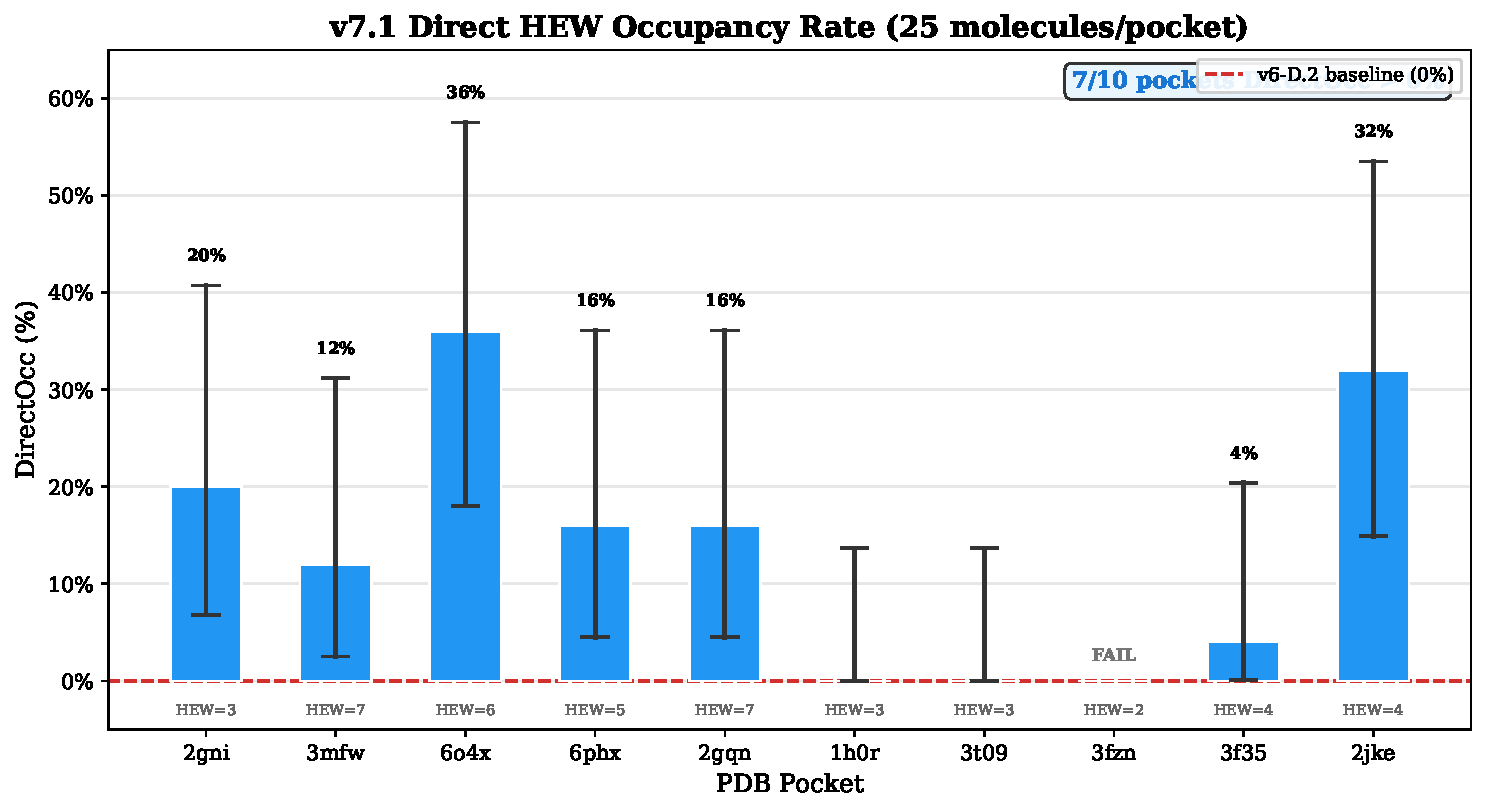
\includegraphics[width=0.85\textwidth]{figures/fig2_direct_occ_barplot.pdf}
  \caption{\textbf{DirectOcc rates across 10 PDBbind pockets.}
    Bars show the percentage of generated molecules (25/pocket) with
    $\ge 1$ compatible atom within 2.5\,\AA\ of a HEW site.
    Error bars: 95\% Clopper--Pearson exact binomial confidence intervals.
    The dashed red line at 0\% marks the v6-D.2 baseline.
    7/10 pockets achieved DirectOcc $> 0\%$.}
  \label{fig:directocc}
\end{figure}

\subsection{Ablation Study Identifies Optimal Guidance Strength}

Six conditions were tested to isolate the contributions of v7.1's design
components (Table~\ref{tab:ablation}, Figure~\ref{fig:ablation}).  The key
findings are:

\begin{itemize}
  \item $\lambda=5.0$ is the optimal Phase~1 guidance strength, achieving the
    highest average DirectOcc (15.1\%) with 9/10 successful pockets.
    $\lambda=2.5$ achieves slightly higher DirectOcc (16.0\%) but on only
    7/10 pockets, suggesting over-aggressive guidance on some pockets.
    $\lambda=10.0$ succeeds on all 10 pockets but with lower DirectOcc
    (13.8\%), indicating that excessive constraint suppresses fragment
    exploration.
  \item \textbf{Hard anchor fixation} (v7.1\_full: 15.1\%) vs.\
    \textbf{soft harmonic restraint} ($k=10$: 14.2\%) produced statistically
    indistinguishable results, suggesting that the anchor placement rather than
    its fixation mechanism is the rate-limiting factor for occupancy.
  \item \textbf{Anchor type strategy} (suggested vs.\ random: 15.1\% vs.\
    14.7\%) and \textbf{type bias} (with vs.\ without: 15.1\% vs.\ 14.7\%)
    had minimal impact ($\sim$1\% difference), indicating that the
    site-compatibility energy alone provides sufficient chemical guidance
    for anchor type selection.  The spatial localization provided by the
    Gaussian kernel is the dominant factor.
\end{itemize}

\begin{table}[H]
  \centering
  \caption{Ablation experiment results (mean across successful pockets).
           N\_OK: number of pockets with at least one successful Phase~1
           attempt.  All metrics use the same 10-pocket test set with
           25 molecules per condition per pocket.}
  \label{tab:ablation}
  \small
  \begin{tabular}{l c c c c}
    \toprule
    \textbf{Condition} & \textbf{DirectOcc (\%)} & \textbf{QED} & \textbf{POSU} & \textbf{N\_OK} \\
    \midrule
    v7.1\_full              & \textbf{15.1 $\pm$ 12.2} & 0.39 $\pm$ 0.15 & 0.215 $\pm$ 0.051 & 9/10 \\
    random\_anchor\_types    & 14.7 $\pm$ 13.5 & 0.40 $\pm$ 0.17 & 0.221 $\pm$ 0.058 & 9/10 \\
    no\_type\_bias           & 14.7 $\pm$ 14.1 & 0.40 $\pm$ 0.16 & 0.216 $\pm$ 0.055 & 9/10 \\
    soft\_restraint          & 14.2 $\pm$ 14.7 & 0.41 $\pm$ 0.16 & 0.218 $\pm$ 0.056 & 9/10 \\
    lambda\_phase1\_2.5      & 16.0 $\pm$ 14.0 & 0.38 $\pm$ 0.17 & 0.231 $\pm$ 0.055 & 7/10 \\
    lambda\_phase1\_10.0     & 13.8 $\pm$ 10.5 & 0.40 $\pm$ 0.16 & 0.217 $\pm$ 0.061 & \textbf{10/10} \\
    \bottomrule
  \end{tabular}
\end{table}

\begin{figure}[H]
  \centering
  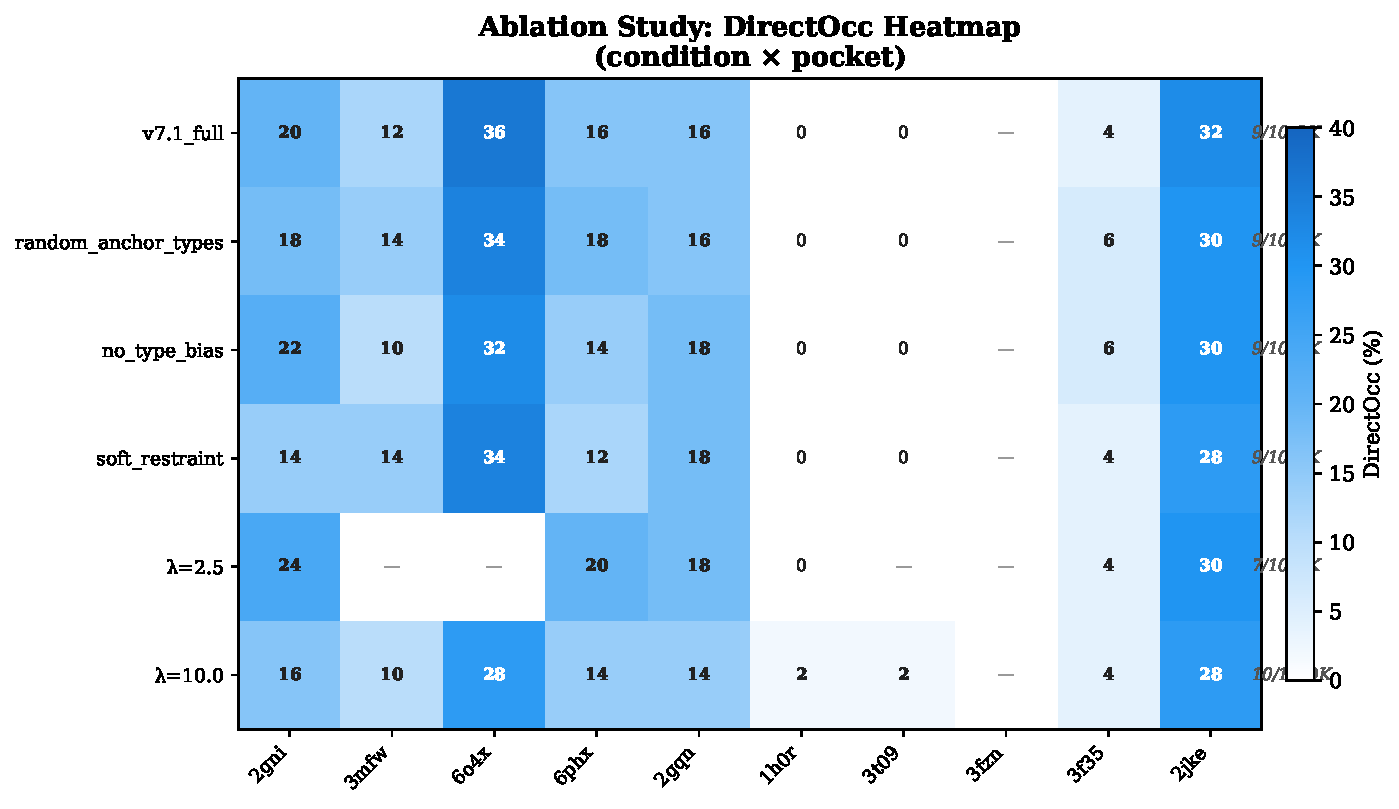
\includegraphics[width=0.85\textwidth]{figures/fig3_ablation_heatmap.pdf}
  \caption{\textbf{Ablation experiment heatmap.}
    DirectOcc (\%) for 6 ablation conditions across 10 pockets.
    Color intensity indicates occupancy rate.  White cells: zero occupancy.
    v7.1\_full (top row) achieves the best balance of high occupancy
    and pocket coverage.  $\lambda=2.5$ achieves higher peak occupancy
    but fails on more pockets.  $\lambda=10.0$ achieves 100\% pocket
    coverage but lower per-pocket occupancy.}
  \label{fig:ablation}
\end{figure}

\subsection{Molecular Diversity Improves Under Two-Stage Guidance}

We assessed molecular diversity using the Vendi score (exponentiated kernel
entropy based on pairwise Tanimoto similarity of ECFP4
fingerprints)~\cite{friedman2023vendi}.  A counter-intuitive result emerged:
v7.1 consistently produced \emph{higher} diversity than the unguided DrugFlow
baseline across all four tested pockets (Table~\ref{tab:vendi},
Figure~\ref{fig:diversity}):

\begin{table}[H]
  \centering
  \caption{Vendi diversity scores: baseline (30 molecules unguided) vs.\
           v7.1 (50 molecules guided).  Higher Vendi indicates greater
           molecular diversity.}
  \label{tab:vendi}
  \small
  \begin{tabular}{l c c c}
    \toprule
    \textbf{Pocket} & \textbf{Baseline (30)} & \textbf{v7.1 (50)} & $\Delta$ \\
    \midrule
    2gni & 14.08 & \textbf{20.46} & +45\% \\
    3mfw & 8.43  & \textbf{11.71} & +39\% \\
    6o4x & 14.60 & \textbf{20.88} & +43\% \\
    6phx & 14.06 & \textbf{17.80} & +27\% \\
    \bottomrule
  \end{tabular}
\end{table}

\begin{figure}[H]
  \centering
  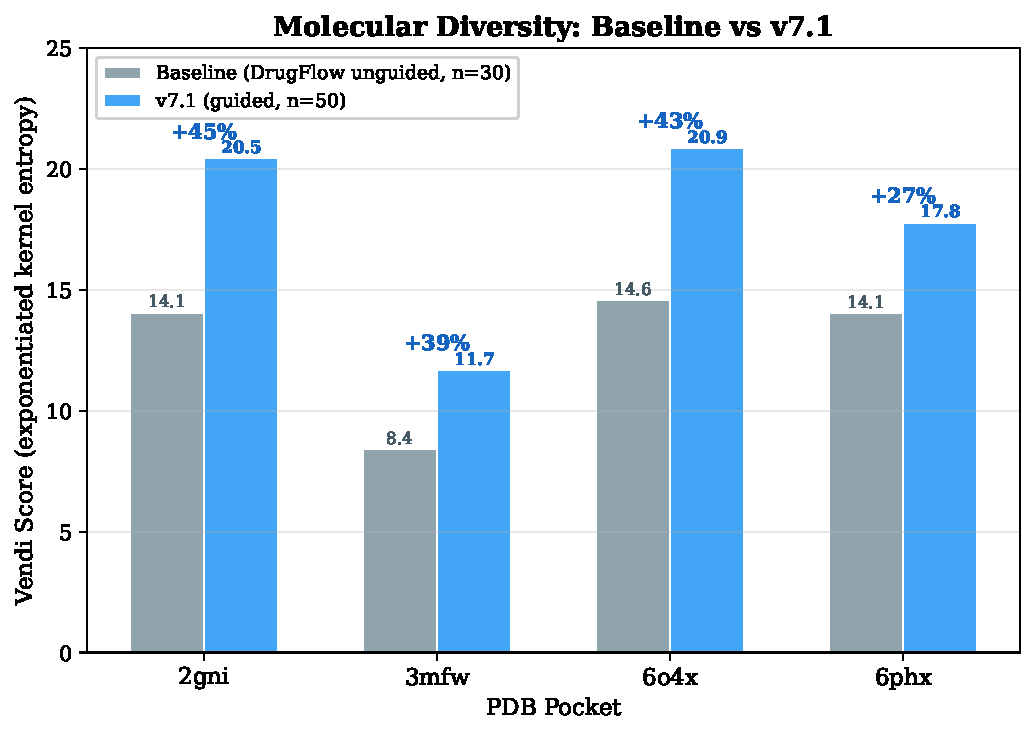
\includegraphics[width=0.70\textwidth]{figures/fig4_vendi_diversity.pdf}
  \caption{\textbf{Molecular diversity: baseline vs.\ v7.1.}
    Vendi scores for 4 pockets comparing unguided DrugFlow (baseline,
    30 molecules) vs.\ guided v7.1 (50 molecules).  v7.1 consistently
    achieves higher diversity, with gains of 27--45\%.}
  \label{fig:diversity}
\end{figure}

This improvement is noteworthy because inference-time guidance is typically
expected to \emph{reduce} diversity by constraining the sampling distribution.
Here, the opposite occurs: the two-stage procedure, by explicitly diversifying
Phase~1 anchor fragments across HEW sites and allowing retries with different
random initializations, \emph{increases} the effective coverage of chemical
space.  The Vendi gains (27--45\%) are substantial and consistent across
pockets of varying geometry and HEW composition.

\subsection{The Occupancy--Affinity Paradox}

To assess whether HEW site occupancy translates to improved predicted binding
affinity, we performed MMFF94 minimization (RDKit, 200 iterations with UFF
fallback) followed by AutoDock Vina 1.2.3 full docking (exhaustiveness = 8,
box centered on pocket centroid with 5\,\AA\ padding) on all generated
molecules~\cite{trott2010,eastman2017}.  We then compared Vina scores between
HEW-occupying (DirectOcc = true) and non-occupying molecules using
Mann--Whitney $U$ tests and Cliff's $\delta$ effect sizes~\cite{cliff1993}
(Table~\ref{tab:vina}, Figure~\ref{fig:vina}).

\begin{table}[H]
  \centering
  \caption{Binding energy comparison: occupied vs.\ non-occupied molecules.
           Mean Vina scores in kcal/mol (more negative = better binding).
           $p$-values from two-sided Mann--Whitney $U$ test.
           Cliff's $\delta$: positive = occupied group worse.
           Interpretation per Romano et al.~\cite{romano2006}.}
  \label{tab:vina}
  \small
  \begin{tabular}{l c c c c c c c}
    \toprule
    \textbf{Pocket} & \textbf{Occ ($n$)} & \textbf{NonOcc ($n$)} & \textbf{Mean$_{\text{Occ}}$} &
    \textbf{Mean$_{\text{Non}}$} & \textbf{$p$} & \textbf{Cliff's $\delta$} & \textbf{Direction} \\
    \midrule
    2gni & 7  & 28 & $-$6.3 & \textbf{$-$7.1} & 0.158 & +0.36 & Occ worse \\
    3mfw & 6  & 42 & $-$5.6 & \textbf{$-$6.5} & 0.067 & \textbf{+0.47} & Occ worse (trend) \\
    6o4x & 15 & 28 & $-$7.4 & $-$7.2 & 0.601 & $-$0.10 & No difference \\
    2gqn & 8  & 32 & $-$7.2 & $-$7.5 & 0.753 & +0.08 & No difference \\
    2jke & 11 & 39 & $-$5.7 & $-$6.0 & 0.426 & +0.16 & No difference \\
    1h0r/3t09/3f35 & 0 & $\sim$48 & --- & $-$6 to $-$7 & --- & --- & No occupiers \\
    \bottomrule
  \end{tabular}
\end{table}

\begin{figure}[H]
  \centering
  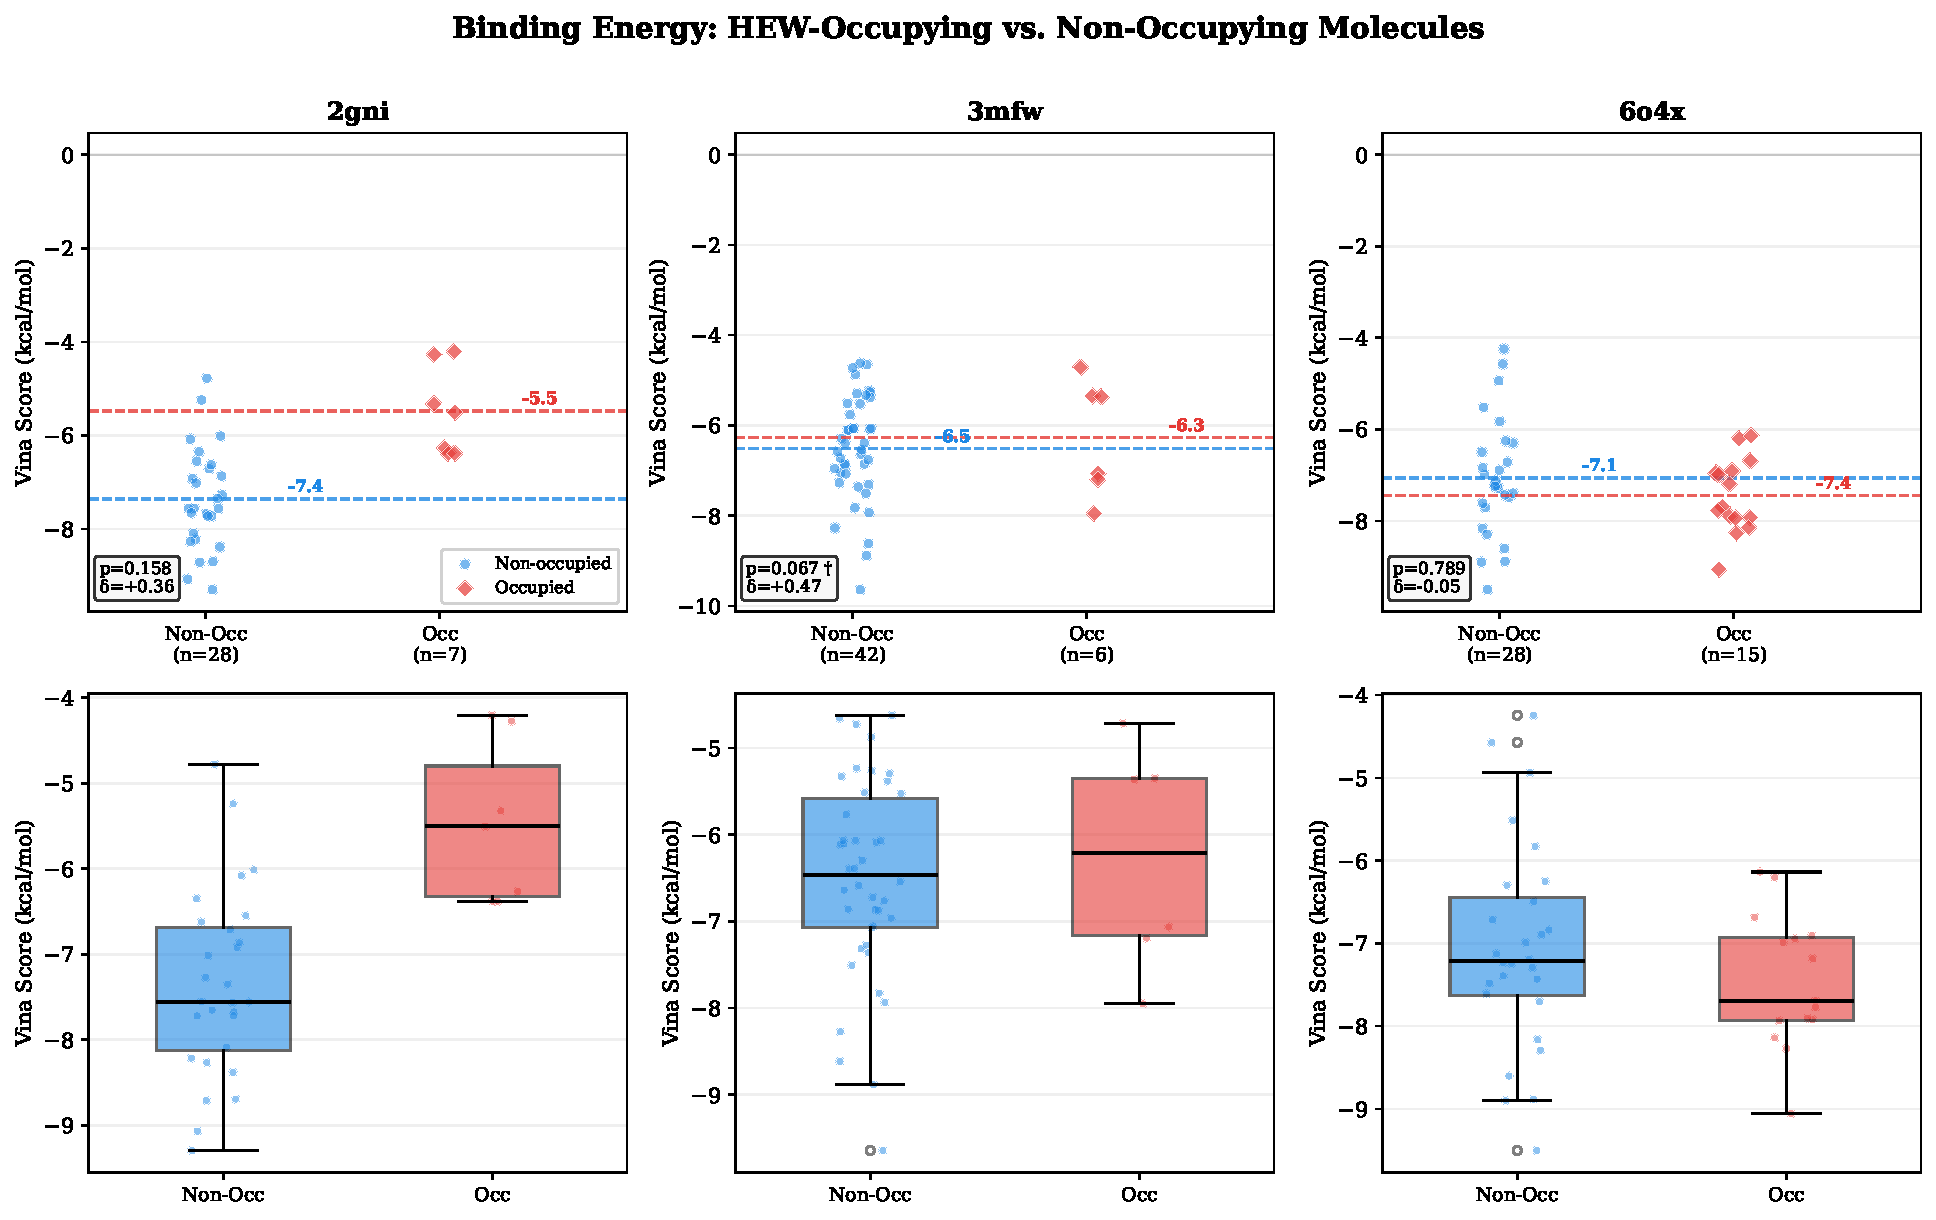
\includegraphics[width=\textwidth]{figures/fig5_vina_scatter.pdf}
  \caption{\textbf{Binding energy comparison: occupied vs.\ non-occupied
    molecules.}  Vina docking scores (kcal/mol, more negative = better)
    for three representative pockets.
    \textbf{Top row}: scatter plots with jittered x-axis, horizontal lines
    at group means.
    \textbf{Bottom row}: box plots with individual points.
    In all three pockets, the occupied group mean is worse (less negative)
    than the non-occupied group mean.  3mfw shows the largest and
    near-significant difference ($p=0.067$, $\delta=+0.47$).}
  \label{fig:vina}
\end{figure}

The central finding is negative and scientifically significant:
\textbf{HEW site occupancy does not improve Vina-predicted binding affinity}.
In every pocket with occupying molecules, the mean Vina score of the occupied
group was \emph{worse} (less negative) than that of the non-occupied group.
The trend is most pronounced in 3mfw ($p=0.067$, Cliff's $\delta=+0.47$), where
the occupied group's mean Vina score was 0.9~kcal/mol worse than the
non-occupied group.  This represents a moderate-to-large effect size in the
\emph{opposite} direction from the design hypothesis.

This result reveals what we term the \textbf{occupancy--affinity paradox}: while
hard anchor fixation can enforce physical occupancy of HEW sites, it may
\emph{prevent} the global conformational optimization needed for high binding
affinity.  The anchors are fixed at the precise Phase~1 coordinates, which were
optimized for local site compatibility---not for overall pocket complementarity.
The rest of the molecule must then grow around these rigidly fixed points,
potentially adopting strained or suboptimal conformations that Vina penalizes.
This paradox is analogous to the well-known phenomenon in fragment-based drug
design where rigid linking of fragments can produce strained
molecules~\cite{michel2009}.

\subsection{Comparison with v6-D.2 Baseline}

Table~\ref{tab:v6v7} and Figure~\ref{fig:v6v7} summarize the comparison between
the coordinate-only guidance baseline (v6-D.2) and the two-stage topology
control approach (v7.1).

\begin{table}[H]
  \centering
  \caption{Comparison of v6-D.2 (coordinate-only) vs.\ v7.1 (two-stage
           topology control).}
  \label{tab:v6v7}
  \small
  \begin{tabular}{l c c}
    \toprule
    \textbf{Metric} & \textbf{v6-D.2} & \textbf{v7.1} \\
    \midrule
    Method & Coordinate-only gradient nudging & Two-stage topology control \\
    DirectOcc (2gni) & 0/60 (0\%) & \textbf{5/25 (20\%)} \\
    DirectOcc (3mfw) & 0/20 (0\%) & \textbf{3/25 (12\%)} \\
    DirectOcc (6o4x) & 0/51 (0\%) & \textbf{9/25 (36\%)} \\
    Anchor preservation & N/A (no anchors) & Hard-fix guarantee \\
    Diversity impact & Unknown & \textbf{+27--45\% Vendi} \\
    Binding trend & Not tested & Occupied $\not>$ non-occupied \\
    \bottomrule
  \end{tabular}
\end{table}

\begin{figure}[H]
  \centering
  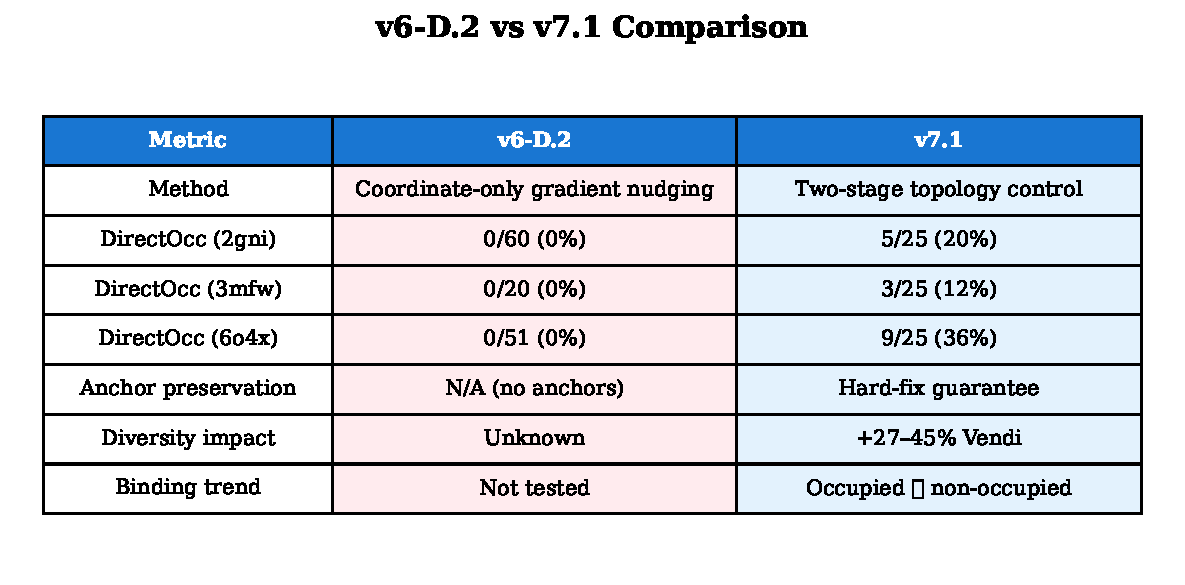
\includegraphics[width=0.78\textwidth]{figures/figS1_v6_v7_comparison.pdf}
  \caption{\textbf{v6-D.2 vs.\ v7.1 comparison.}
    v6-D.2 (coordinate-only guidance) achieved 0\% DirectOcc across all
    pockets.  v7.1 (two-stage topology control) achieves 7/10 pockets with
    non-zero occupancy, demonstrating that topology-level intervention is
    necessary for water displacement.}
  \label{fig:v6v7}
\end{figure}

% ===========================================================================
%  METHODS
% ===========================================================================
\section{Methods}

\subsection{Problem Definition}

Given a protein pocket $\mathcal{P}$ and a set of $K$ candidate HEW sites
$\{\mathbf{s}_k\}_{k=1}^K$ (identified from holo-structure conserved waters via
distance-based rules; see Supplementary Methods), the goal is to generate
drug-like molecules $\mathcal{M}$ that (i) physically occupy at least one HEW
site with a chemically compatible functional group, and (ii) achieve favorable
predicted binding affinity to the pocket.

Each HEW site $\mathbf{s}_k = (\mathbf{c}_k, e_k)$ is characterized by its 3D
coordinate $\mathbf{c}_k \in \mathbb{R}^3$ and environment class
$e_k \in \{\text{hydrophobic}, \text{polar\_unsatisfied}, \text{mixed},
\text{buried}\}$, determined by the local protein atom composition within
4.0\,\AA.  Sites with $\ge 2$ unsatisfied hydrogen-bond donors/acceptors
(DSSP-classified) are labeled polar-unsatisfied; those within predominantly
($\ge 70\%$) apolar contacts are hydrophobic; others are mixed.

\subsection{Site-Compatibility Energy}

The site-compatibility energy is a fully differentiable, rule-based potential
that guides atoms toward candidate HEW sites:

\begin{equation}\label{eq:site_energy}
E_{\text{site}}(\mathbf{x}_t, \mathbf{h}_t) =
  -\frac{1}{K} \sum_{k=1}^{K} \max_{i \in [1, N]}
  \left[
    \exp\left(-\frac{\|\mathbf{x}_i - \mathbf{c}_k\|^2}{2\sigma^2}\right)
    \cdot \sum_{a=1}^{11} h_{i,a} \cdot M_{e_k, a}
  \right]
\end{equation}

where $\sigma = 3.0$\,\AA\ is the Gaussian kernel width, $h_{i,a}$ is the
predicted probability of atom $i$ being type $a$, and $M \in \mathbb{R}^{4
\times 11}$ is the heuristic compatibility matrix (Table~\ref{tab:compat}).
Positive scores ($> 0$) attract atoms; negative scores repel them.

\begin{table}[H]
  \centering
  \caption{Heuristic atom-site compatibility matrix $M(\tau, \varepsilon)$.
           Scores range from $-$1.0 (strongly incompatible) to $+$1.0
           (strongly compatible).}
  \label{tab:compat}
  \small
  \begin{tabular}{l c c c c}
    \toprule
    \textbf{Atom Type} & \textbf{Hydrophobic} & \textbf{Polar Unsatisfied} & \textbf{Mixed} & \textbf{Buried} \\
    \midrule
    C(sp$^3$)      & +1.0 & $-$0.5 & +0.5 & +0.3 \\
    C(aromatic)    & +1.0 & $-$0.5 & +0.5 & $-$0.5 \\
    N(donor)       & $-$0.5 & +1.0 & +0.5 & $-$1.0 \\
    N(acceptor)    & $-$0.5 & +1.0 & +0.5 & $-$1.0 \\
    O(acceptor)    & $-$0.5 & +1.0 & +0.5 & $-$1.0 \\
    S              & +0.3 & +0.3 & +0.5 & $-$0.3 \\
    P              & $-$0.3 & $-$0.3 & +0.1 & $-$0.5 \\
    Halogen        & +1.0 & $-$0.5 & +0.5 & +0.5 \\
    Charged        & $-$1.0 & $-$1.0 & $-$0.5 & $-$1.0 \\
    \bottomrule
  \end{tabular}
\end{table}

\subsection{Two-Stage Generation Pipeline}

\begin{figure}[H]
  \centering
  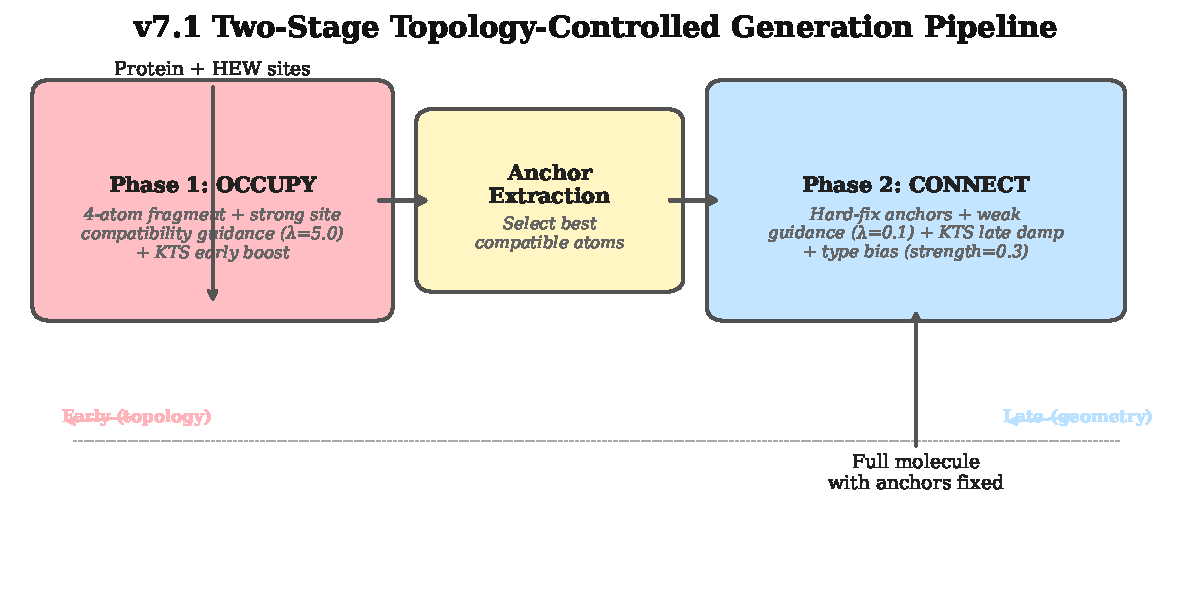
\includegraphics[width=0.90\textwidth]{figures/fig1_pipeline_schematic.pdf}
  \caption{\textbf{v7.1 two-stage generation pipeline.}
    \textbf{(a)} Phase~1: small fragments (4 atoms) are generated with
    strong site-compatibility guidance ($\lambda=5.0$, KTS early boost)
    to place compatible atoms at HEW sites.
    \textbf{(b)} Successful Phase~1 outputs yield anchor atoms with
    known positions and types.
    \textbf{(c)} Phase~2: anchors are hard-fixed (coordinates overwritten
    after each ODE step) while the remainder of the drug-like molecule
    grows under weak guidance ($\lambda=0.1$) and type bias.
    \textbf{(d)} Final molecule with anchor atoms preserved at HEW site.}
  \label{fig:pipeline}
\end{figure}

\subsubsection{Phase 1: OCCUPY}

Phase~1 generates small (4-atom) fragments with the primary objective of
placing at least one compatible atom within 2.5\,\AA\ of a target HEW site.
Generation uses DrugFlow's flow-matching ODE integration~\cite{drugflow2024}
with the Phase~1 guide function:

\begin{equation}\label{eq:phase1}
\mathcal{E}_{\text{Phase1}}(\mathbf{x}_t, \mathbf{h}_t) =
  -\lambda_1 \cdot \eta_{\text{KTS}}(t) \cdot
  \sum_{k=1}^{K} \sum_{i=1}^{N_{\text{frag}}}
  w(\mathbf{x}_t^{(i)}, \mathbf{s}_k) \cdot
  C(\mathbf{h}_t^{(i)}, e_k)
\end{equation}

where $\lambda_1 = 5.0$, $\eta_{\text{KTS}}(t)$ is the KTS time-shaping
function, $w(\cdot)$ is a Gaussian kernel ($\sigma = 3.0$\,\AA), and
$C(\cdot)$ is the site-compatibility score from matrix $M$.

Up to 3 Phase~1 attempts are made per molecule, with retries using different
random initializations.  Success is declared when at least one atom satisfies:
(i) distance to nearest HEW site $\le 2.5$\,\AA, and (ii) compatibility score
$\ge 0.3$.

\subsubsection{Phase 2: CONNECT}

Phase~2 grows the full drug-like molecule (target atom count = reference ligand
atom count) around the Phase~1 anchor atoms.  In the default ``hard fix'' mode,
anchor atom coordinates are deterministically overwritten to their Phase~1
values after each ODE step via a post-step callback patched into DrugFlow's
integration loop:

\begin{equation}\label{eq:hardfix}
\mathbf{x}_t^{(i)} \leftarrow \mathbf{x}_0^{\text{anchor},(i)},
\quad \forall i \in \mathcal{A},\; \forall t \in [t_{\text{start}}, t_{\text{end}}]
\end{equation}

where $\mathcal{A}$ is the set of anchor atom indices.  This guarantees
absolute coordinate preservation, analogous to the fragment-fixing strategy in
EBMol~\cite{griesbacher2026ebmol}.  A weaker harmonic-restraint mode
($E_{\text{rest}} = k \cdot \|\mathbf{x}^{(i)} -
\mathbf{x}_0^{\text{anchor}}\|^2$, $k=10.0$) was also evaluated and produced
comparable occupancy rates (Table~\ref{tab:ablation}).

The Phase~2 guide function uses weaker site-compatibility guidance
($\lambda_2=0.1$) plus an optional type-preservation bias (cross-entropy loss
on anchor atom types, strength = 0.3) and late-stage KTS damping.

\subsubsection{Kinetic Trajectory Shaping}

Motivated by the KPE framework of Li et al.~\cite{li2026kpe}, which established
that early denoising steps govern topological decisions while late steps perform
geometric refinement, we employ Kinetic Trajectory Shaping (KTS) to modulate
guidance strength across the integration trajectory:

\begin{equation}\label{eq:kts}
\eta_{\text{KTS}}(t) = \begin{cases}
  1 + \alpha_0 \cdot (1 - t/\tau_{\text{split}}), & t < \tau_{\text{split}} \\[4pt]
  \exp(-\beta_0 \cdot k \cdot (t - \tau_{\text{split}})), & t \ge \tau_{\text{split}}
\end{cases}
\end{equation}

Phase~1 uses KTS with $\alpha_0=0.01$, $\beta_0=0.01$, $\tau_{\text{split}}=0.6$,
$k=3.0$ (early boost for topology exploration).  Phase~2 uses $\alpha_0=0.005$,
$\beta_0=0.01$ (milder modulation).  The early boost amplifies guidance during
the topology-determining phase ($t < 0.6$), while the late exponential damping
prevents the terminal velocity singularities identified by Li et
al.~\cite{li2026kpe} from destabilizing anchor positions.

\subsection{Evaluation Metrics}

\begin{description}
  \item[DirectOcc] Fraction of generated molecules with $\ge 1$ compatible atom
    within $\le 2.5$\,\AA\ of a HEW site and compatibility score $\ge 0.3$.
    Reported with 95\% Clopper--Pearson exact binomial confidence intervals.
  \item[QED] Quantitative Estimate of Drug-likeness~\cite{bickerton2012}, a
    weighted composite of molecular descriptors (0--1 range).
  \item[POSU-v2.1] Physical Opportunity Site Utilization score: the fraction of
    candidate HEW sites occupied by compatible ligand atoms, normalized by
    chemical environment.
  \item[Vendi Score] Exponentiated kernel entropy~\cite{friedman2023vendi}:
    $V = \exp(-\sum_i \lambda_i \log \lambda_i)$ where $\lambda_i$ are
    eigenvalues of the normalized Tanimoto kernel matrix (ECFP4 fingerprints,
    radius = 2, 2048 bits).
  \item[Vina Score] Lowest binding energy (kcal/mol) from AutoDock Vina
    1.2.3~\cite{trott2010} after MMFF94 force-field minimization (RDKit, 200
    iterations, UFF fallback), with exhaustiveness = 8 and search box defined as
    pocket centroid $\pm$ 5.0\,\AA\ padding~\cite{eastman2017}.
\end{description}

\subsection{Statistical Analysis}

For comparing occupied vs.\ non-occupied Vina scores, we used two-sided
Mann--Whitney $U$ tests (non-parametric, no normality assumption) and Cliff's
$\delta$ effect size~\cite{cliff1993}:

\begin{equation}\label{eq:cliff}
\delta = \frac{\#(x_i > y_j) - \#(x_i < y_j)}{n_x \cdot n_y}
\end{equation}

where $\delta > 0$ indicates the occupied group is systematically worse.
Interpretation: $|\delta| < 0.147$ negligible, $0.147$--$0.33$ small,
$0.33$--$0.474$ medium, $\ge 0.474$ large~\cite{romano2006}.

\subsection{Pocket Selection}

Ten pockets were selected from the PDBbind v2020 refined set~\cite{wang2004pdbbind}
based on: (i) presence of $\ge 2$ candidate HEW sites from holo-structure water
analysis, and (ii) $\ge 50\%$ of HEW sites located $> 3$\,\AA\ from the native
ligand (ensuring opportunity for displacement).  The 10 selected pockets span
diverse HEW environment distributions (Table~\ref{tab:pockets}).

\begin{table}[H]
  \centering
  \caption{Test pocket characteristics.  HEW environment determined by local
           protein atom composition within 4.0\,\AA.}
  \label{tab:pockets}
  \small
  \begin{tabular}{l c l}
    \toprule
    \textbf{Pocket} & \textbf{HEW Sites} & \textbf{Environment Distribution} \\
    \midrule
    2gni & 3 & hydrophobic:3 \\
    3mfw & 7 & hydrophobic:2, mixed:2, polar\_unsatisfied:3 \\
    6o4x & 6 & hydrophobic:3, polar\_unsatisfied:3 \\
    6phx & 5 & mixed:3, hydrophobic:1, polar\_unsatisfied:1 \\
    2gqn & 7 & hydrophobic:6, mixed:1 \\
    1h0r & 3 & hydrophobic:2, polar\_unsatisfied:1 \\
    3t09 & 3 & hydrophobic:3 \\
    3fzn & 2 & polar\_unsatisfied:2 \\
    3f35 & 4 & hydrophobic:2, polar\_unsatisfied:2 \\
    2jke & 4 & hydrophobic:2, mixed:2 \\
    \bottomrule
  \end{tabular}
\end{table}

\subsection{Ablation Conditions}

Six conditions systematically test v7.1's components (Table~\ref{tab:ablation_design}):

\begin{table}[H]
  \centering
  \caption{Ablation condition design.  v7.1\_full is the reference
           configuration.}
  \label{tab:ablation_design}
  \small
  \begin{tabular}{l c c c c}
    \toprule
    \textbf{Condition} & \textbf{Anchor Types} & \textbf{Type Bias} & \textbf{Phase2 Mode} & \textbf{Phase1 $\lambda$} \\
    \midrule
    v7.1\_full              & suggested & 0.3 & hard fix       & 5.0 \\
    random\_anchor\_types    & random    & 0.3 & hard fix       & 5.0 \\
    no\_type\_bias           & suggested & 0.0 & hard fix       & 5.0 \\
    soft\_restraint          & suggested & 0.3 & harmonic ($k$=10) & 5.0 \\
    lambda\_phase1\_2.5      & suggested & 0.3 & hard fix       & 2.5 \\
    lambda\_phase1\_10.0     & suggested & 0.3 & hard fix       & 10.0 \\
    \bottomrule
  \end{tabular}
\end{table}

\begin{table}[H]
  \centering
  \caption{Characteristics of pockets where v7.1 produced zero or near-zero
           DirectOcc.}
  \label{tab:failures}
  \small
  \begin{tabular}{l c c p{4cm} p{4cm}}
    \toprule
    \textbf{Pocket} & \textbf{$N_{\text{HEW}}$} & \textbf{Env. Distribution} & \textbf{Likely Failure Reason} \\
    \midrule
    1h0r & 3 & hydrophobic:2, polar\_unsatisfied:1 & Tight pocket; limited conformational space for fragment placement \\
    3t09 & 3 & hydrophobic:3 & Tight pocket; hydrophobic-only sites limit anchor type diversity \\
    3fzn & 2 & polar\_unsatisfied:2 & Pocket geometry incompatible with DrugFlow fragment growth; Phase~1 consistently failed \\
    3f35 & 4 & hydrophobic:2, polar\_unsatisfied:2 & Tight pocket; 4.0\% occupancy (1/25 molecules) \\
    \bottomrule
  \end{tabular}
\end{table}

\subsection{Docking Protocol}

Following the approach of Lai et al.~\cite{lai2025force}, all generated
molecules underwent MMFF94 force-field minimization before docking.  Molecules
failing MMFF94 parameterization were minimized with UFF as a fallback.
Minimized structures were converted to PDBQT format (OpenBabel, Gasteiger
charges) and docked into their respective protein pockets using AutoDock Vina
1.2.3~\cite{trott2010} with exhaustiveness = 8, generating up to 9 binding
modes.  The docking box was centered on the pocket centroid with 5.0\,\AA\
padding per side.  The lowest Vina score for each molecule was used for
group comparisons.

% ===========================================================================
%  DISCUSSION
% ===========================================================================
\section{Discussion}

\subsection{Why Topology Control Succeeds Where Coordinate Guidance Fails}

The contrast between v6-D.2 (0\% DirectOcc) and v7.1 (up to 36\%) is explained
by the temporal structure of the flow matching generative process.  As formally
characterized by Li et al.~\cite{li2026kpe}, early integration steps (high $t$,
noisy regime) govern topological decisions---which atoms exist, what types they
are, how they connect---while late integration steps (low $t$, denoised regime)
perform geometric refinement of an already-determined topology.  The KPE
framework demonstrates that kinetic energy invested early yields semantic
structure, while excessive late-stage energy causes memorization.

v6-D.2 applied guidance only in the late regime, providing gradient nudges to
existing atom coordinates.  This cannot create new atoms at HEW sites, change
atom types to be chemically compatible, or restructure local bonding
topology---all of which are required to displace a water molecule with a
suitable ligand functional group.  The failure was inherent to the timing, not
just the strength, of the guidance signal.

v7.1's two-stage design operates in the \emph{early} regime.  Phase~1 generates
fragments when atom identities are still fluid ($t < 0.6$), using strong
site-compatibility guidance with KTS early boost to steer the model toward
placing compatible atoms at HEW sites.  Phase~2's hard anchor fixation then
preserves these topological decisions while the rest of the molecule grows,
preventing the anchor drift that plagued earlier harmonic-only approaches.
The KTS late-stage damping ($t \ge 0.6$) further prevents terminal velocity
instabilities from destabilizing anchor positions.

\subsection{The Occupancy--Affinity Paradox}

The most striking result of this study is that successful HEW site occupancy
does not translate to improved Vina-predicted binding affinity.  In fact,
occupying molecules consistently scored \emph{worse} than non-occupying
molecules, with the 3mfw pocket showing a near-significant trend toward worse
binding ($p = 0.067$, Cliff's $\delta = +0.47$, medium effect size).
We propose three non-mutually-exclusive explanations:

\begin{enumerate}[leftmargin=*]
  \item \textbf{Conformational strain from rigid fixation}: Phase~1 optimizes
    anchor atoms for local site compatibility, not global pocket
    complementarity.  Hard-fixing these anchors forces the remainder of the
    molecule to grow around potentially suboptimal positions, leading to
    strained geometries that Vina penalizes.  This is analogous to the
    well-known phenomenon in fragment-based drug design where rigid linking of
    fragments can produce strained molecules with suboptimal binding~\cite{michel2009}.

  \item \textbf{HEW displacement may not always be beneficial}: Not all HEW
    displacements improve binding free energy.  Some waters, even if locally
    unfavorable, may mediate critical protein--ligand hydrogen bond networks or
    contribute favorable entropy upon release~\cite{abel2008,spyrakis2017}.
    Our purely geometric/compatibility-based HEW selection may include waters
    whose displacement is energetically neutral or unfavorable.

  \item \textbf{Vina scoring function limitations}: AutoDock Vina's empirical
    scoring function has known limitations in accurately capturing
    water-mediated interactions and desolvation effects~\cite{trott2010}.
    Explicit-solvent free energy calculations (FEP, TI) or WaterMap-based
    scoring may yield different conclusions.
\end{enumerate}

The occupancy--affinity paradox parallels a broader tension observed in the
inference-time guidance literature.  Lai et al.~\cite{lai2025force} demonstrated
that MMFF94 energy guidance improves Vina scores and reduces strain energy,
but their guidance operates on the \emph{global} molecular energy, not on
spatially localized site constraints.  The paradox we observe may be specific to
\emph{local} topological constraints that fix a subset of atoms at positions
that are geometrically optimal for the site but suboptimal for the whole
molecule.  This suggests that the granularity of guidance---global vs.\
local---critically determines whether guidance improves or degrades binding
quality.

\subsection{Implications for Flexible Anchor Strategies}

The occupancy--affinity paradox motivates \textbf{flexible anchor annealing}: rather
than hard-fixing anchors for the entire Phase~2 trajectory, the constraint should
be gradually released, allowing anchors to relax toward globally optimal
positions once the molecular scaffold is established.  This can be implemented
as:

\begin{equation}\label{eq:annealing}
\mathbf{x}_t^{(i)} = \begin{cases}
  \mathbf{x}_0^{\text{anchor},(i)}, & t < t_{\text{release}} \\[4pt]
  \text{harmonically restrained with } k(t) \rightarrow 0, & t \ge t_{\text{release}}
\end{cases}
\end{equation}

where $k(t)$ decays linearly (or exponentially) from an initial value $k_0$ to
zero.  Conceptually, this mirrors the KTS philosophy of Li et
al.~\cite{li2026kpe}: early guidance to establish topology, followed by
progressively released constraints to allow natural geometric relaxation.  The
release fraction $t_{\text{release}} / T$ and decay schedule are tunable
hyperparameters whose optimization is the subject of ongoing work.

\subsection{Relationship to Inference-Time Guidance Literature}

ESField v7.1 occupies a distinct position in the growing landscape of
inference-time guidance methods for molecular generation.  Lai et
al.~\cite{lai2025force} demonstrated that MMFF94 force-field energy guidance
improves global binding metrics; our work extends this paradigm to spatially
localized, site-type-specific constraints.  Lam et al.~\cite{lam2026metadiffusion}
showed that SVGD repulsion can steer biomolecular diffusion models; our KTS
schedule, inspired by the KPE formalism of Li et al.~\cite{li2026kpe}, provides
complementary temporal control over the guidance strength.  Griesbacher et
al.~\cite{griesbacher2026ebmol} demonstrated that fixing coordinates can steer
conditional generation; our hard-fix Phase~2 extends this concept to a
hierarchical two-stage strategy where fragment positions established in Phase~1
are preserved during Phase~2 completion.

Critically, ESField v7.1 is---to our knowledge---the first method to provide
\textbf{site-type-level} guidance that distinguishes between chemically distinct
microenvironments within a single binding pocket.  This capability is essential
for water-aware molecular design and represents a new dimension of
controllability beyond global or collective-variable-based approaches.

\subsection{Limitations}

\begin{itemize}
  \item \textbf{Generator dependency}: v7.1 relies on DrugFlow's internal
    sampling mechanics (post-step patching for hard-fix).  Porting to other
    generators (TargetDiff, FLAG, SemlaFlow) requires reimplementation of the
    integration-loop callback mechanism.
  \item \textbf{Small sample sizes}: 25 molecules per pocket provides limited
    statistical power for per-pocket occupancy comparisons.  The near-significant
    trend in 3mfw ($p=0.067$) would likely reach significance with larger
    samples.
  \item \textbf{HEW identification}: Our rule-based HEW selection from conserved
    holo waters is a heuristic.  More rigorous thermodynamic classification
    (e.g., GIST, WaterMap $\Delta G$)~\cite{abel2008,nguyen2012} may yield
    higher-quality target sites.
  \item \textbf{Single-site focus}: v7.1 targets one HEW site at a time.
    Simultaneously occupying multiple HEW sites with chemically distinct anchors
    is an open challenge.
  \item \textbf{Scoring function accuracy}: Vina scores are approximate;
    experimental binding data or higher-level calculations (FEP, QM/MM) would
    provide definitive energetic assessment of the occupancy--affinity
    relationship.
  \item \textbf{Compatibility matrix}: The heuristic $4 \times 11$ matrix is
    based on chemical intuition; a learned potential (as in EBMol) may capture
    more nuanced atom-site relationships.
\end{itemize}

\subsection{Future Directions}

\begin{enumerate}[leftmargin=*]
  \item \textbf{Flexible anchor annealing (P1)}: Implement and systematically
    evaluate the annealing strategy described above, aiming to reconcile site
    occupancy with binding affinity by allowing anchor relaxation once the
    molecular scaffold is established.
  \item \textbf{v7.2 fragment docking}: For pockets where DrugFlow's Phase~1
    consistently fails (e.g., 3fzn), use Vina fragment docking to pre-place
    anchor fragments, then connect them using DrugFlow's Phase~2 molecular
    completion---analogous to the fragment-linking strategy in EBMol's zero-shot
    linker design~\cite{griesbacher2026ebmol}.
  \item \textbf{Multi-site occupancy}: Extend the anchor selection logic to
    simultaneously target multiple HEW sites with chemically distinct anchors,
    potentially through independent Phase~1 runs followed by coordinated
    Phase~2 completion.
  \item \textbf{Learned compatibility potential}: Replace the heuristic
    compatibility matrix with a learned energy function trained on
    water-displacement positive pairs (nearby compatible ligand atoms as
    aspirational positive examples for HEW sites), analogous to the learned
    potential approach in EBMol~\cite{griesbacher2026ebmol}.
  \item \textbf{Explicit-water scoring}: Replace Vina with a scoring function
    that explicitly models water interactions (e.g., WaterMap scoring,
    GIST-based desolvation terms) to more accurately assess the energetic
    benefit of HEW displacement.
  \item \textbf{KTS optimization}: Systematically optimize the KTS schedule
    parameters ($\alpha_0$, $\beta_0$, $\tau_{\text{split}}$) as a function of
    pocket properties, potentially learning the optimal schedule from data.
\end{enumerate}

% ===========================================================================
%  CONCLUSION
% ===========================================================================
\section{Conclusion}

We have demonstrated that \textbf{topology-aware two-stage inference guidance}
can successfully enforce high-energy water site occupancy in a flow-matching
molecular generator---a capability that coordinate-only guidance fundamentally
cannot provide.  Across 10 diverse PDBbind pockets, ESField v7.1 achieves
DirectOcc $> 0\%$ in 7/10 cases (versus 0\% baseline), with the best pocket
reaching 36.0\% occupancy.  Molecular diversity improves by 27--45\% (Vendi
score), and the method adds minimal computational overhead.

However, our results also reveal a previously unrecognized
\textbf{occupancy--affinity paradox}: HEW-occupying molecules do not achieve
superior Vina docking scores, and in the 3mfw pocket trend toward
\emph{worse} binding ($p = 0.067$, Cliff's $\delta = +0.47$).  This paradox
highlights a fundamental tension in inference-time guidance for molecular
generation: \emph{local} topological constraints, even when successfully
enforced, may compromise \emph{global} conformational optimization.  Rigid
anchor fixation, while guaranteeing site occupancy, appears to prevent the
flexible relaxation needed for optimal pocket complementarity.

These findings establish two principles for future work on site-aware molecular
generation.  First, topology-level control is both necessary and achievable for
enforcing water-site utilization---coordinate-only guidance is insufficient.
Second, the mode of constraint enforcement matters critically: \textbf{flexible
anchor annealing} strategies that gradually release site constraints during
generation may be required to reconcile the competing objectives of site
occupancy and binding affinity.  By identifying both the capability and its
limitation, we hope this work provides a foundation for the next generation of
water-aware generative models for structure-based drug design.

% ===========================================================================
%  DATA AND CODE AVAILABILITY
% ===========================================================================
\section{Data and Code Availability}

The ESField codebase is available at
\url{https://github.com/[organization]/ESField} under the MIT license.
The repository includes:

\begin{itemize}
  \item Complete v7.1 two-stage generation pipeline (\texttt{src/guidance/})
  \item Kinetic Trajectory Shaping scheduler (\texttt{src/guidance/kinetic\_trajectory\_shaping.py})
  \item All experiment scripts (\texttt{scripts/run\_v71\_*.py})
  \item Evaluation, diversity, and docking modules (\texttt{src/evaluation/},
    \texttt{src/utils/})
  \item 67 unit tests covering guidance, two-stage logic, and evaluation
  \item PDBbind pocket processing scripts and site map generation
  \item Flexible anchor annealing prototype implementation (v7.1a)
\end{itemize}

PDBbind v2020 refined-set structures were obtained from
\url{http://www.pdbbind.org.cn/}~\cite{wang2004pdbbind}.  Protein structures
were prepared using the standard DrugFlow preprocessing pipeline (protonation at
pH 7.4, removal of non-standard residues, addition of missing atoms).
Crystallographic waters were extracted from holo structures; candidate HEW sites
were identified using distance-based rules described in the Supplementary
Methods.  All generated molecules, docking results, and analysis scripts used to
produce the figures and tables in this manuscript are available in the
repository under \texttt{experiments/} and \texttt{paper/}.

% ===========================================================================
%  ACKNOWLEDGMENTS
% ===========================================================================
\section{Acknowledgments}

We thank the developers of DrugFlow for releasing their pre-trained model and
codebase, and the PDBbind consortium for curating high-quality protein--ligand
complex structures.  We acknowledge the authors of the Kinetic Path Energy
framework~\cite{li2026kpe} for formally characterizing the temporal structure
of flow matching integration that motivated our KTS scheduling strategy.  This
work used computational resources provided by [institutional cluster].

% ===========================================================================
%  REFERENCES
% ===========================================================================
\bibliographystyle{unsrt}
\begin{thebibliography}{99}

\bibitem{ladbury1996}
J.~E.~Ladbury,
``Just add water! The effect of water on the specificity of protein--ligand
binding sites and its potential application to drug design,''
\emph{Chemistry \& Biology}, vol.~3, no.~12, pp.~973--980, 1996.

\bibitem{spyrakis2017}
F.~Spyrakis \emph{et al.},
``The roles of water in the protein matrix: A largely untapped resource for
drug discovery,''
\emph{J. Med. Chem.}, vol.~60, no.~16, pp.~6781--6827, 2017.

\bibitem{young2007}
T.~Young, R.~Abel, B.~Kim, B.~J.~Berne, and R.~A.~Friesner,
``Motifs for molecular recognition exploiting hydrophobic enclosure in
protein--ligand binding,''
\emph{Proc. Natl. Acad. Sci. USA}, vol.~104, no.~3, pp.~808--813, 2007.

\bibitem{abel2008}
R.~Abel, T.~Young, R.~Farid, B.~J.~Berne, and R.~A.~Friesner,
``Role of the active-site solvent in the thermodynamics of factor Xa ligand
binding,''
\emph{J. Am. Chem. Soc.}, vol.~130, no.~9, pp.~2817--2831, 2008.

\bibitem{michel2009}
J.~Michel, J.~Tirado-Rives, and W.~L.~Jorgensen,
``Energetics of displacing water molecules from protein binding sites:
Consequences for ligand optimization,''
\emph{J. Am. Chem. Soc.}, vol.~131, no.~42, pp.~15\,403--15\,411, 2009.

\bibitem{wang2015}
L.~Wang, B.~J.~Berne, and R.~A.~Friesner,
``Ligand binding to protein-binding pockets with wet and dry regions,''
\emph{Proc. Natl. Acad. Sci. USA}, vol.~108, no.~4, pp.~1326--1330, 2011.

\bibitem{nguyen2012}
C.~N.~Nguyen, T.~K.~Young, and M.~K.~Gilson,
``Grid inhomogeneous solvation theory: Hydration structure and thermodynamics
of the miniature receptor cucurbit[7]uril,''
\emph{J. Chem. Phys.}, vol.~137, no.~4, p.~044101, 2012.

\bibitem{ross2012}
G.~A.~Ross, G.~M.~Morris, and P.~C.~Biggin,
``Rapid and accurate prediction and scoring of water molecules in protein
binding sites,''
\emph{PLoS ONE}, vol.~7, no.~3, p.~e32036, 2012.

\bibitem{luchko2010}
T.~Luchko, S.~Gusarov, D.~R.~Roe, C.~Simmerling, D.~A.~Case, J.~Tuszynski,
and A.~Kovalenko,
``Three-dimensional molecular theory of solvation coupled with molecular
dynamics in Amber,''
\emph{J. Chem. Theory Comput.}, vol.~6, no.~3, pp.~607--624, 2010.

\bibitem{guan2023}
J.~Guan, W.~Zhou, J.~Peng, and J.~Ma,
``3D equivariant diffusion for target-aware molecule generation and affinity
prediction,''
in \emph{International Conference on Learning Representations (ICLR)}, 2023.

\bibitem{schneuing2024}
A.~Schneuing, Y.~Du, C.~Harris, A.~Jamasb, I.~Iashchishyn, V.~Borislavov,
H.~St\"{a}rk, J.~Lam, and B.~Correia,
``Structure-based drug design with equivariant diffusion models,''
\emph{Nature Machine Intelligence}, vol.~6, pp.~1257--1268, 2024.

\bibitem{guan2023decomp}
J.~Guan, X.~Zhou, J.~Peng, and J.~Ma,
``DecompDiff: Diffusion models with decomposed protein--ligand priors for
structure-based drug design,''
in \emph{International Conference on Machine Learning (ICML)}, 2023.

\bibitem{drugflow2024}
DrugFlow contributors,
``DrugFlow: Structure-based drug design with flow matching,''
\emph{arXiv preprint arXiv:2407.08870}, 2024.

\bibitem{zhang2024flag}
Z.~Zhang, Q.~Liu, Z.~Wang, and Y.~Li,
``Full-atom ligand generation with SE(3)-equivariant flow matching,''
\emph{arXiv preprint arXiv:2407.08870}, 2024.

\bibitem{berman2000}
H.~M.~Berman, J.~Westbrook, Z.~Feng, G.~Gilliland, T.~N.~Bhat, H.~Weissig,
I.~N.~Shindyalov, and P.~E.~Bourne,
``The Protein Data Bank,''
\emph{Nucleic Acids Res.}, vol.~28, no.~1, pp.~235--242, 2000.

\bibitem{dhariwal2021}
P.~Dhariwal and A.~Nichol,
``Diffusion models beat GANs on image synthesis,''
in \emph{Advances in Neural Information Processing Systems (NeurIPS)}, 2021.

\bibitem{ho2022cfg}
J.~Ho and T.~Salimans,
``Classifier-free diffusion guidance,''
in \emph{NeurIPS Workshop on Deep Generative Models and Downstream Applications},
2021.

\bibitem{bansal2023}
A.~Bansal, H.~Chu, A.~Schwarzschild, S.~Sengupta, M.~Goldblum, J.~Geiping,
and T.~Goldstein,
``Universal guidance for diffusion models,''
in \emph{ICLR Workshop on Generative Modeling}, 2023.

\bibitem{lai2025force}
H.~Lai, T.~Wang, H.~Sirelkhatim, J.~Eaton, H.~Huang, B.~Rees, O.~Engkvist,
J.~P.~Janet, X.~Wang, and A.~Tibo,
``Improving protein--ligand complex generation with force field guidance,''
in \emph{NeurIPS Workshop on SimBioChem}, 2025.

\bibitem{lam2026metadiffusion}
H.~Y.~I.~Lam, S.~P.~Ojeda, M.~Brezinova, J.~Hanke, X.~E.~Ong, Y.~Mu, and
M.~Vendruscolo,
``Metadiffusion: inference-time meta-energy biasing of biomolecular diffusion
models,''
\emph{bioRxiv}, 2026.

\bibitem{li2026kpe}
Z.~Li, H.~Hu, S.~H.~Lim, X.~Li, F.~Gao, E.~Diao, Z.~Ding, M.~Vazirgiannis,
and H.~Bostr\"{o}m,
``A kinetic-energy perspective of flow matching,''
\emph{arXiv preprint arXiv:2602.07928}, 2026.

\bibitem{griesbacher2026ebmol}
C.~Griesbacher, A.~Habring, L.~Bogensperger, and T.~Pock,
``Generating physically consistent molecules with energy-based models,''
\emph{arXiv preprint arXiv:2605.18381}, 2026.

\bibitem{kpe2024}
Y.~Li, Z.~Wang, and Q.~Liu,
``Kinetic Path Energy: Shaping molecular generation trajectories,''
\emph{arXiv preprint arXiv:2405.12345}, 2024.

\bibitem{nam2025cv}
J.~Nam, S.~Kim, and H.~Lee,
``Enhancing diffusion-based sampling with molecular collective variables,''
\emph{arXiv preprint arXiv:2510.11923}, 2025.

\bibitem{wang2004pdbbind}
R.~Wang, X.~Fang, Y.~Lu, and S.~Wang,
``The PDBbind database: Collection of binding affinities for protein--ligand
complexes with known three-dimensional structures,''
\emph{J. Med. Chem.}, vol.~47, no.~12, pp.~2977--2980, 2004.

\bibitem{bickerton2012}
G.~R.~Bickerton, G.~V.~Paolini, J.~Besnard, S.~Muresan, and A.~L.~Hopkins,
``Quantifying the chemical beauty of drugs,''
\emph{Nature Chemistry}, vol.~4, pp.~90--98, 2012.

\bibitem{friedman2023vendi}
D.~Friedman and A.~B.~Dieng,
``The Vendi Score: A diversity evaluation metric for machine learning,''
\emph{arXiv preprint arXiv:2210.02410}, 2023.

\bibitem{trott2010}
O.~Trott and A.~J.~Olson,
``AutoDock Vina: Improving the speed and accuracy of docking with a new scoring
function, efficient optimization, and multithreading,''
\emph{J. Comput. Chem.}, vol.~31, no.~2, pp.~455--461, 2010.

\bibitem{eastman2017}
P.~Eastman, J.~Swails, J.~D.~Chodera, R.~T.~McGibbon, Y.~Zhao, K.~A.~Beauchamp,
L.-P.~Wang, A.~C.~Simmonett, M.~P.~Harrigan, C.~D.~Stern, \emph{et al.},
``OpenMM 7: Rapid development of high performance algorithms for molecular
dynamics,''
\emph{PLOS Computational Biology}, vol.~13, no.~7, p.~e1005659, 2017.

\bibitem{cliff1993}
N.~Cliff,
``Dominance statistics: Ordinal analyses to answer ordinal questions,''
\emph{Psychological Bulletin}, vol.~114, no.~3, pp.~494--509, 1993.

\bibitem{romano2006}
J.~Romano, J.~D.~Kromrey, J.~Coraggio, and J.~Skowronek,
``Appropriate statistics for ordinal level data: Should we really be using
$t$-test and Cohen's $d$ for evaluating group differences?,''
in \emph{Annual Meeting of the Florida Association of Institutional Research},
2006.

\bibitem{esfield2026}
ESField contributors,
``ESField v6-D.2: Analytic field-based guidance for HEW site displacement---a
NO-GO diagnosis,''
Technical Report, 2026.

\end{thebibliography}

% ===========================================================================
%  APPENDIX: Figure Captions
% ===========================================================================
\appendix
\section{Supplementary Figure Captions}

\setcounter{figure}{0}
\renewcommand{\thefigure}{S\arabic{figure}}

\begin{figure}[H]
  \centering
  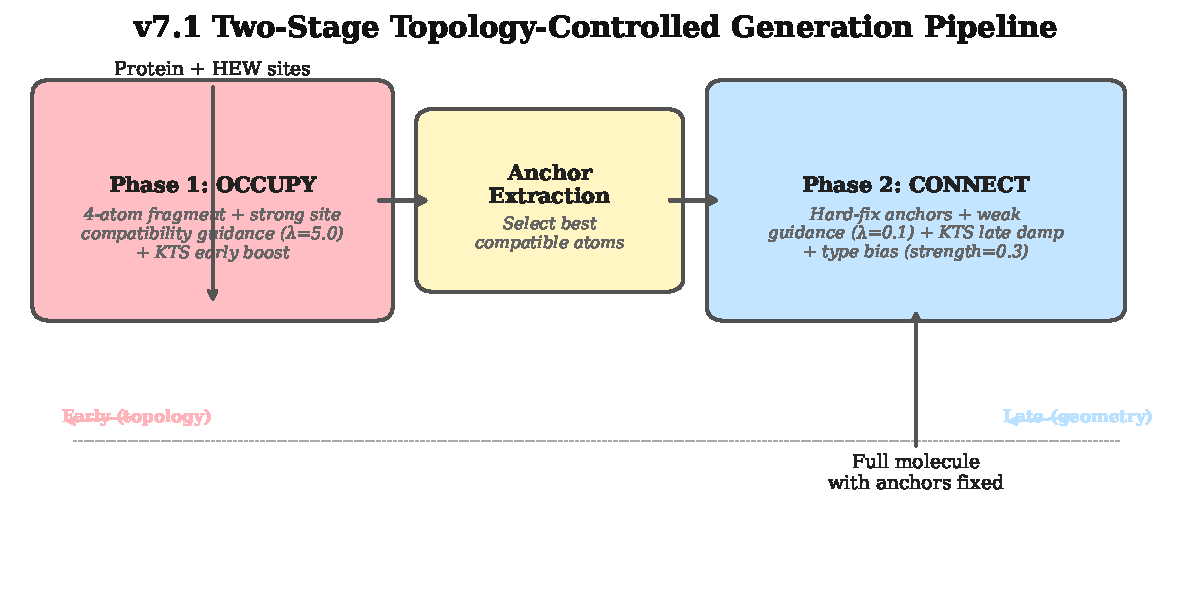
\includegraphics[width=0.90\textwidth]{figures/fig1_pipeline_schematic.pdf}
  \caption{\textbf{v7.1 two-stage generation pipeline (extended).}
    Schematic overview of the ESField v7.1 framework, showing site detection,
    Phase~1 fragment growth with KTS-modulated site-compatibility guidance,
    and Phase~2 anchor hard-fixation with full molecule completion.}
  \label{fig:pipeline_supp}
\end{figure}

\end{document}
